\documentclass[12pt]{article}
%\usepackage[cp1251]{inputenc}
\usepackage[utf8]{inputenc}
\usepackage[bulgarian]{babel}
\usepackage{amssymb,amsmath,amsfonts,amstext,amscd,latexsym}
\usepackage{graphicx}
\usepackage{amsmath}
\usepackage[colorinlistoftodos]{todonotes}
\usepackage{systeme}
\usepackage[geometry]{ifsym}
\usepackage{listings}
\usepackage{float}
\usepackage{color}

\begin{document}
	\begin{titlepage}	
		\newcommand{\HRule}{\rule{\linewidth}{0.5mm}} % Defines a new command for the horizontal lines, change thickness here
		\begin{center}
		\textsc{\LARGE Софийски университет }\\[0.3cm]
		\textsc{\LARGE "Св. Климент Охридски" }\\[0.3cm]
		\textsc{\Large Факултет по математика и информатика }\\[0.2cm]
		%\fontsize{size}{baselineskip}
		
		{\fontsize{12}{18}\selectfont \bf МАШИННО САМООБУЧЕНИЕ}\vspace{15pt}\newline спец. Изкуствен интелект, I курс, зимен семестър \newline учебна година 2024/2025
		\vspace{30pt}
		
		
		
		
		
		\begin{minipage}{0.4\textwidth}
			\begin{flushleft}\large
				\emph{Изготвил:} \\
				Кристиян Симов \\ 
				фак. номер 4MI3400288
			\end{flushleft}
		\end{minipage}
		~
		%\begin{flushleft}
		\begin{minipage}{0.4\textwidth}
			\begin{flushright}
				\large
				\emph{Дата:}\\
				25. 10. 2024 г. % Попълнете датата на предаване
				\\София 
			\end{flushright}
		\end{minipage}\\[1cm]
		%\end{flushleft}
		\bigskip
		{\large \textbf{Домашна работа \textnumero 2}}\\[1cm] % Date, change the \today to a set date if you want to be precise
		%\includegraphics{rsz_sofia_university_logo.png}\\[1cm] 
		
\includegraphics{logo_su_no_text.png}\\[1cm]
		\vfill % Fill the rest of the page with whitespace
		\end{center}
	\end{titlepage}
	
	
	
	\tableofcontents
	
	
	
	\newpage
	
	\section{Решение на задача \textnumero 1}
	
	
	Нека имаме множество от обучаващи примери $S$ дефинирано чрез таблицата:
	\newline
	\begin{table}[h!]
	\centering
		\begin{tabular}{|c|c|c|c|}
			\hline
			Пример & Класификация & $A_{1}$ & $A_{2}$ \\ \hline				1      & +            & T       & T       \\ \hline
			2      & +            & T       & T       \\ \hline
			3      & -            & T       & F       \\ \hline
			4      & +            & F       & F       \\ \hline
			5      & -            & F       & T       \\ \hline
			6      & -            & F       & T       \\ \hline
		\end{tabular}
	\end{table}
	\newline
	
	\paragraph{a)}
	Формулата за изчисление на ентропия от информационната теория за произволно множество от примери $S$ с булеви стойности на целевата функция (+ или -) , показваща неговата еднородност, е:
	
	\begin{center}
		$Entropy(S) \equiv -p_{+}\log_2 p_{+} - p_{-}\log_2 p_{-}$,
	\end{center}
	където $p_{+}$ и $p_{-}$ са съответно отношенията на броя на положителните и отрицателните примери към броят всички примери.\newline\newline
	Прилагаме я към конкретното множество S и последователно получаваме:
	
	\begin{center}
	$Entropy([3_{+}, 3_{-}]) = -\frac{3}{6}\log_2 \frac{3}{6} - \frac{3}{6}\log_2 \frac{3}{6} = -\frac{1}{2}\log_2 \frac{1}{2} - \frac{1}{2}\log_2 \frac{1}{2} =\newline\newline= -\frac{1}{2}(-1) - \frac{1}{2}(-1) = \frac{1}{2} + \frac{1}{2} = 1$
	\end{center}
	Очаквано, получихме ентропия равна на 1, тъй като броят на положителните и отрицателните примери е еднакъв (в случая равен на 3).\newline
	\newpage
	\paragraph{b)}
	Формулата за изчисление информационната печалба на атрибут $A$ по отношение на произволно множество от примери $S$ е:
	
	\begin{center}
		$Gain(S, A) \equiv Entropy(S) - \displaystyle\sum_{v \in Values(A)} \frac{|S_{v}|}{|S|}Entropy(S_{v})$,
	\end{center}
	където $Values(A)$ е множеството от възможни стойности на атрибута $A$, а множеството $S_{v} = \{ s \in S | A(s) = v \}$.\newline\newline
	Прилагаме я към атрибута $A_{2}$ по отношение на конкретното множество S и последователно получаваме:
	
	\begin{center}
		$Gain(S, A_{2}) = Entropy(S) - \displaystyle\sum_{v \in Values(A_{2})} \frac{|S_{v}|}{|S|}Entropy(S_{v}) =$\newline
		$= 1 - \displaystyle\sum_{v \in \{T, F\}} \frac{|S_{v}|}{6}Entropy(S_{v}) =$\newline
		$= 1 - \frac{|S_{T}|}{6}Entropy(S_{T}) - \frac{|S_{F}|}{6}Entropy(S_{F}) =$
		$ = 1 - (\frac{4}{6})1 - (\frac{2}{6})1 = 0$
	\end{center}
	Очаквано, получихме печалба равна на 0, тъй като броят на положителните и отрицателните примери е еднакъв в подмножествата $S_{T}$ и $S_{F}$.\newline
	\newpage
	
	\section{Решение на задача \textnumero 2}
	\paragraph{a)}
	
	Нека имаме множество от обучаващи примери $S$ дефинирано чрез таблицата:
	\newline
	\begin{table}[!h]
	\centering
		\begin{tabular}{|c|c|c|c|c|c|c|c|}
			\hline
			\textit{Пример} & \textit{Небе} & \textit{Въздух} & \textit{Влажност} & \textit{Вятър} & \textit{Вода} & \textit{Прогноза} & \textit{Харесва} \\ \hline
			1               & Слънце        & Топъл           & Нормална          & Силен          & Топла         & Същото            & \textbf{Да}      \\ \hline
			2               & Слънце        & Топъл           & Висока            & Силен          & Топла         & Същото            & \textbf{Да}      \\ \hline
			3               & Дъжд          & Студен          & Висока            & Силен          & Топла         & Промяна           & \textbf{Не}      \\ \hline
			4               & Слънце        & Топъл           & Висока            & Силен          & Студена       & Промяна           & \textbf{Да}      \\ \hline
		\end{tabular}
	\end{table}
	\newline\newline
	Тогава алгоритъмът ID3 ще премине през следните стъпки:\newline
	
	
	\paragraph{0)} $S = \{x_{1}, x_{2}, x_{3}, x_{4}\},  A = \{A_{\textnormal{Небе}},  A_{\textnormal{Въздух}}, A_{\textnormal{Влажност}}, A_{\textnormal{Вятър}}, A_{\textnormal{Вода}}, A_{\textnormal{Прогноза}}\}$
	\subparagraph{}
	$Entropy(S) = -p_{+}\log_2 p_{+} - p_{-}\log_2 p_{-} = -\frac{3}{4}\log_2 \frac{3}{4} - \frac{1}{4}\log_2 \frac{1}{4} \approx 0.811 $
	\subparagraph{}
	$Gain(A_{\textnormal{Небе}}, S) \approx 0.811 - (0 + 0) = 0.811 \leftarrow best$
	\subparagraph{}
	$Gain(A_{\textnormal{Въздух}}, S) = Gain(A_{\textnormal{Небе}}, S) \approx 0.811$
	\subparagraph{}
	$Gain(A_{\textnormal{Влажност}}, S) \approx 0.811 - (0 + \frac{3}{4}*0.918) \approx 0.811 - 0.689 = 0.122$
	\subparagraph{}
	$Gain(A_{\textnormal{Вятър}}, S) \approx 0.811 - 0.811 = 0$
	\subparagraph{}
	$Gain(A_{\textnormal{Вода}}, S) = A_{\textnormal{Влажност}}, S) \approx 0.122$
	\subparagraph{}
	$Gain(A_{\textnormal{Прогноза}}, S) \approx 0.811 - (0 + \frac{2}{4}*1) = 0.811 - 0.5 = 0.311$
	\newpage
	
	\paragraph{1)}
	 $S_{\textnormal{Слънце}} = \{x_{1}, x_{2}, x_{4}\},  A = \{A_{\textnormal{Небе}},  A_{\textnormal{Въздух}}, A_{\textnormal{Влажност}}, A_{\textnormal{Вятър}}, A_{\textnormal{Вода}}, A_{\textnormal{Прогноза}}\}$
	\subparagraph{}
	$Entropy(S_{\textnormal{Слънце}}) = -p_{+}\log_2 p_{+} - p_{-}\log_2 p_{-} = -\frac{3}{3}0  - \frac{0}{3}1 = 0 - 0 = 0$
	\subparagraph{}
	Множеството $S_{\textnormal{Слънце}}$ е напълно еднородно - образуваме листо със
	\subparagraph{} знак "Да".

	\paragraph{2)}
	$S_{\textnormal{Дъжд}} = \{x_{3}\},  A = \{A_{\textnormal{Небе}},  A_{\textnormal{Въздух}}, A_{\textnormal{Влажност}}, A_{\textnormal{Вятър}}, A_{\textnormal{Вода}}, A_{\textnormal{Прогноза}}\}$
	\subparagraph{}
	$Entropy(S_{\textnormal{Облаци}}) = -p_{+}\log_2 p_{+} - p_{-}\log_2 p_{-} = -\frac{0}{1}1  - \frac{1}{1}0 = 0 - 0 = 0$
	\subparagraph{}
	Множеството $S_{\textnormal{Дъжд}}$ е напълно еднородно - образуваме листо със
	\subparagraph{} знак "Не".
	\newline\newline
	Край - дървото е обучено и изглежда така:
	\newline
		\begin{figure}[H]
		\centering
		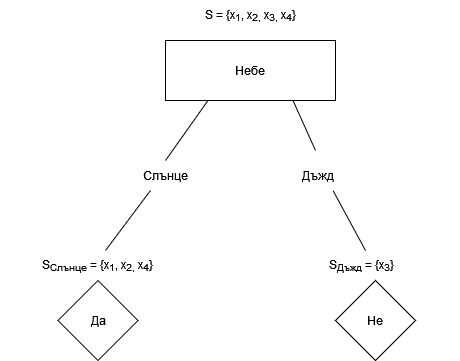
\includegraphics[width=80mm]{Untitled Diagram1.png} 
		\caption{На изображението виждаме, че още след първото най-добро разделяне дървото е обучено успешно.}
	\end{figure}

	\paragraph{b)}
	
	Нека към предходната таблица за $S$ прибавим още един обучаващ пример:
	\newline
	\begin{table}[!h]
		\centering
		\begin{tabular}{|c|c|c|c|c|c|c|c|}
			\hline
			\textit{Пример} & \textit{Небе} & \textit{Въздух} & \textit{Влажност} & \textit{Вятър} & \textit{Вода} & \textit{Прогноза} & \textit{Харесва} \\ \hline
			1               & Слънце        & Топъл           & Нормална          & Силен          & Топла         & Същото            & \textbf{Да}      \\ \hline
			2               & Слънце        & Топъл           & Висока            & Силен          & Топла         & Същото            & \textbf{Да}      \\ \hline
			3               & Дъжд          & Студен          & Висока            & Силен          & Топла         & Промяна           & \textbf{Не}      \\ \hline
			4               & Слънце        & Топъл           & Висока            & Силен          & Студена       & Промяна           & \textbf{Да}      \\ \hline
			5               & Слънце        & Топъл           & Нормална            & Слаб          & Топла       & Същото           & \textbf{Не}      \\ \hline
		\end{tabular}
	\end{table}
	\newline\newline
	Тогава алгоритъмът ID3 ще премине през следните стъпки:\newline
	
	
	\paragraph{0)} $S = \{x_{1}, x_{2}, x_{3}, x_{4}, x_{5}\},  A = \{A_{\textnormal{Небе}},  A_{\textnormal{Въздух}}, A_{\textnormal{Влажност}}, A_{\textnormal{Вятър}}, A_{\textnormal{Вода}}, A_{\textnormal{Прогноза}}\}$
	\subparagraph{}
	$Entropy(S) = -p_{+}\log_2 p_{+} - p_{-}\log_2 p_{-} = -\frac{3}{5}\log_2 \frac{3}{5} - \frac{2}{5}\log_2 \frac{2}{5} \approx 0.970 $
	\subparagraph{}
	$Gain(A_{\textnormal{Небе}}, S) \approx 0.970 - (0 + \frac{4}{5}*0.811) = 0.970 - 0.608 = 0.362 \leftarrow best$
	\subparagraph{}
	$Gain(A_{\textnormal{Въздух}}, S) = Gain(A_{\textnormal{Небе}}, S) \approx 0.362$
	\subparagraph{}
	$Gain(A_{\textnormal{Влажност}}, S) \approx 0.970 - (\frac{2}{5}*1 + \frac{3}{5}*0.918) \approx 0.970 - 0.951 = 0.019$
	\subparagraph{}
	$Gain(A_{\textnormal{Вятър}}, S) \approx 0.970 - (\frac{1}{5}*0 + \frac{4}{5}*0.811) = 0.970 - 0.649 = 0.321$
	\subparagraph{}
	$Gain(A_{\textnormal{Вода}}, S) = \approx 0.970 - (\frac{1}{5}*0 + \frac{4}{5}*1) = 0.970 - 0.8 = 0.170$
	\subparagraph{}
	$Gain(A_{\textnormal{Прогноза}}, S) = Gain(A_{\textnormal{Влажност}}, S) \approx 0.019$
	\newpage
	
	\paragraph{1)}
	$S_{\textnormal{Слънце}} = \{x_{1}, x_{2}, x_{4}, x_{5}\},  A = \{A_{\textnormal{Небе}},  A_{\textnormal{Въздух}}, A_{\textnormal{Влажност}}, A_{\textnormal{Вятър}}, A_{\textnormal{Вода}}, A_{\textnormal{Прогноза}}\}$
	\subparagraph{}
	$Entropy(S_{\textnormal{Слънце}}) = -\frac{3}{4}\log_2 \frac{3}{4}  - \frac{1}{4}\log_2 \frac{1}{4} \approx 0.811$
	\subparagraph{}
	$Gain(A_{\textnormal{Небе}}, S) \approx 0.811 - 0.811 = 0$
	\subparagraph{}
	$Gain(A_{\textnormal{Въздух}}, S) = Gain(A_{\textnormal{Небе}}, S) = 0$
	\subparagraph{}
	$Gain(A_{\textnormal{Влажност}}, S) \approx 0.811 - (\frac{2}{4}*0 + \frac{2}{4}*1) \approx 0.811 - 0.5 = 0.311$
	\subparagraph{}
	$Gain(A_{\textnormal{Вятър}}, S) \approx 0.811 - (\frac{1}{4}*1 + \frac{3}{4}*0) = 0.811 - 0.25 = 0.561 \leftarrow best$
	\subparagraph{}
	$Gain(A_{\textnormal{Вода}}, S) = \approx 0.811 - (\frac{1}{4}*0 + \frac{3}{4}*0.918) = 0.970 - 0.689 = 0.122$
	\subparagraph{}
	$Gain(A_{\textnormal{Прогноза}}, S) = Gain(A_{\textnormal{Вода}}, S) \approx 0.122$
	
	
	\paragraph{2)}
	$S_{\textnormal{Силен}} = \{x_{1}, x_{2}, x_{4}\},  A = \{A_{\textnormal{Небе}},  A_{\textnormal{Въздух}}, A_{\textnormal{Влажност}}, A_{\textnormal{Вятър}}, A_{\textnormal{Вода}}, A_{\textnormal{Прогноза}}\}$
	\subparagraph{}
	$Entropy(S_{\textnormal{Силен}}) = -p_{+}\log_2 p_{+} - p_{-}\log_2 p_{-} = -\frac{3}{3}0  - \frac{0}{3}1 = 0 - 0 = 0$
	\subparagraph{}
	Множеството $S_{\textnormal{Силен}}$ е напълно еднородно - образуваме листо със
	\subparagraph{} знак "Да".
	
	\paragraph{3)}
	$S_{\textnormal{Слаб}} = \{x_{5}\},  A = \{A_{\textnormal{Небе}},  A_{\textnormal{Въздух}}, A_{\textnormal{Влажност}}, A_{\textnormal{Вятър}}, A_{\textnormal{Вода}}, A_{\textnormal{Прогноза}}\}$
	\subparagraph{}
	$Entropy(S_{\textnormal{Слаб}}) = -p_{+}\log_2 p_{+} - p_{-}\log_2 p_{-} = -\frac{0}{1}1  - \frac{1}{1}0 = 0 - 0 = 0$
	\subparagraph{}
	Множеството $S_{\textnormal{Слаб}}$ е напълно еднородно - образуваме листо със
	\subparagraph{} знак "Не".
	
	\paragraph{4)}
	$S_{\textnormal{Дъжд}} = \{x_{3}\},  A = \{A_{\textnormal{Небе}},  A_{\textnormal{Въздух}}, A_{\textnormal{Влажност}}, A_{\textnormal{Вятър}}, A_{\textnormal{Вода}}, A_{\textnormal{Прогноза}}\}$
	\subparagraph{}
	$Entropy(S_{\textnormal{Дъжд}}) = -p_{+}\log_2 p_{+} - p_{-}\log_2 p_{-} = -\frac{0}{1}1  - \frac{1}{1}0 = 0 - 0 = 0$
	\subparagraph{}
	Множеството $S_{\textnormal{Дъжд}}$ е напълно еднородно - образуваме листо със
	\subparagraph{} знак "Не".
	\newline\newline
	Край - дървото е обучено и изглежда така:
	\newline
	\begin{figure}[H]
		\centering
		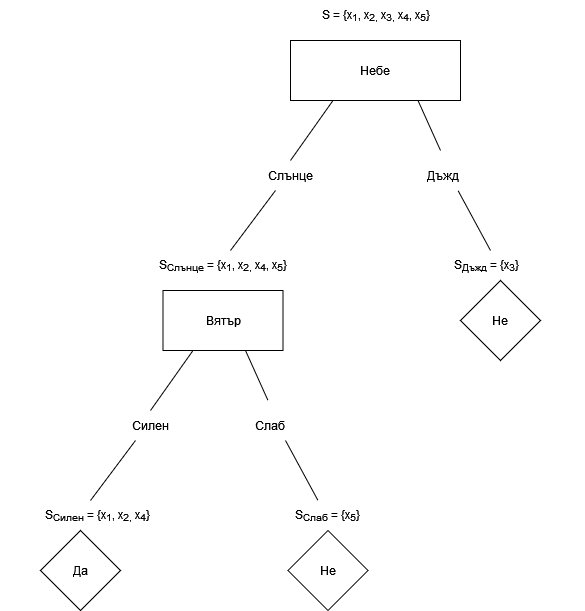
\includegraphics[width=120mm]{Untitled Diagram2.png} 
		\caption{На изображението виждаме, че вече след първото най-добро разделяне се налага да изберем още едно такова за множеството в лявото поддърво, след което дървото е обучено успешно.}
	\end{figure}
		
	\newpage
	
	\section{Решение на задача \textnumero 3}
	
	\paragraph{a)} $A \land \neg B$
		\begin{figure}[H]
			\centering
			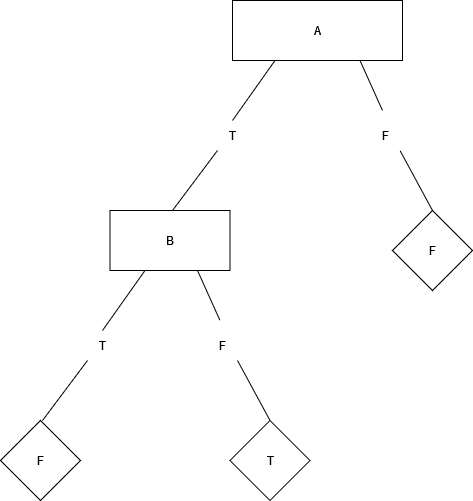
\includegraphics[width=120mm]{Untitled Diagram3.png} 
			\caption{a)}
		\end{figure}
	
	\newpage
	
	\paragraph{b)} $A \lor (B \land C)$
	\begin{figure}[H]
		\centering
		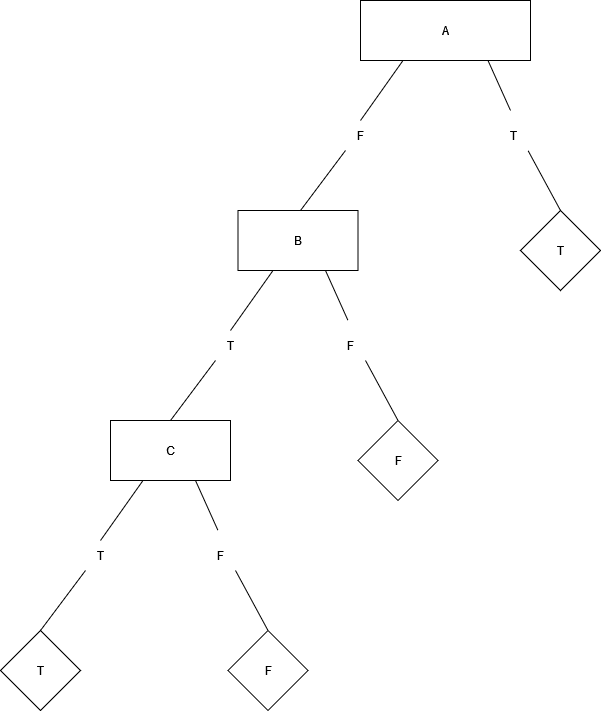
\includegraphics[width=120mm]{Untitled Diagram4.png} 
		\caption{b)}
	\end{figure}

	\newpage

	\paragraph{c)} $(A \land B) \lor (C \land D)$
	\begin{figure}[H]
		\centering
		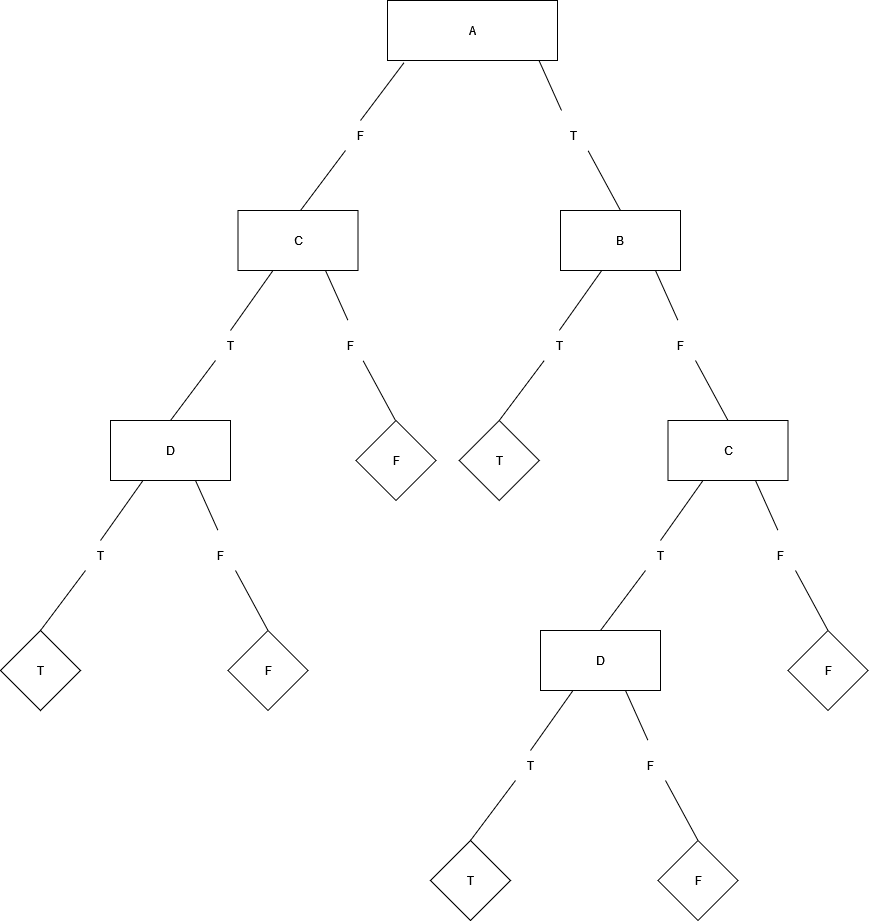
\includegraphics[width=150mm]{Untitled Diagram5.png} 
		\caption{c)}
	\end{figure}
	
	\newpage
	
	\section{Решение на задача \textnumero 4}
	
	Нека D1 и D2 са класификационни дървета описващи булеви функции (като тези от Задача \textnumero 3), такива че D2 е получено от D1 чрез заместване на листо (термален възел) в D1 с цяло поддърво T'.\newline
	\newline
	Ще покажем, че твърдението:
	\subparagraph{}
	\textit{D1 e \textbf{по-общо-или-равно-на} D2}
	\newline\newline
	е \textbf{не}винаги в сила.
	
	\paragraph{1)} Нека за простота D1 се описва чрез израза:
	\subparagraph{}
	$A$
	\subparagraph{}
	Тогава D1 ще изглежда така:
	
	\begin{figure}[H]
		\centering
		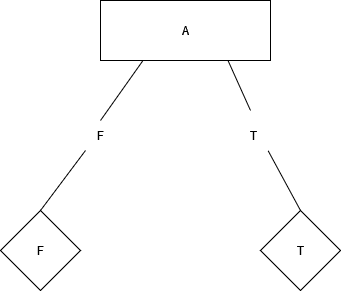
\includegraphics[width=60mm]{Untitled Diagram8.png} 
		\caption{D1}
	\end{figure}
	
	\paragraph{1)} Нека получим израз за D2 от този на D1 чрез добавяне на непразния (състоящ се поне от променлива B) израз на поддърво $T'$ посредством дизюнкция:
	\subparagraph{}
	$A \lor T'$
	\subparagraph{}
	Тогава D2 най-общо ще изглежда така:
	
	\begin{figure}[H]
		\centering
		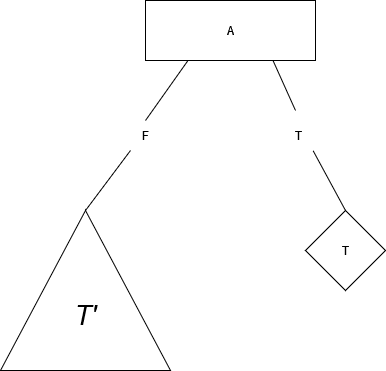
\includegraphics[width=80mm]{Untitled Diagram9.png} 
		\caption{D2}
	\end{figure}
	
	Забелязваме, че вече оценката на пример с $A = F$ не е директно F, а вече зависи от резултата от минаването по поддървото $T'$. Ако резултатът от това минаване е Т, тогава общия резултат ще е Т противно на резултатът F, получен при $A = F$ в D1. Tова би означавало противоречие с твърдението, тъй като примерът $A = F \land T' = T$ се покрива от хипотезата D2, но не от хипотезата D1. Нека за простота изразът описващ поддървото $T'$ е равен на B. Тоест израза за D2 става:
	\subparagraph{}
	$A \lor B$
	\newline\newline
	Тогава D2 ще изглежда по следния начин:
	\begin{figure}[H]
		\centering
		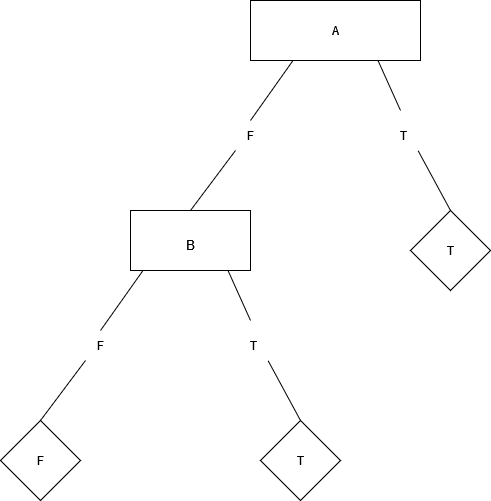
\includegraphics[width=80mm]{Untitled Diagram10.png} 
		\caption{D2}
	\end{figure}
	
	Нека разгледаме примерът $x \equiv A = F \land B = T$. Той се покрива от хипотезата D2 ($D2(x) = T$), но не се покрива от хипотезата D1 ($D1(x) = F$). D1 го "изпуска". Достигнахме до противоречие с твърдението \textit{D1 e \textbf{по-общо-или-равно-на} D2}. $\square$
	
\end{document}